\documentclass[12 pt, a4paper]{article}
\usepackage[english]{babel}  								% For norsk oppsett
\usepackage[utf8]{inputenc}
\usepackage{amsmath}
\usepackage{amssymb}
\usepackage{graphicx}
\usepackage{tabularx}
\usepackage{subcaption}
\usepackage{hyperref}
\usepackage{fancyhdr}
\usepackage{enumerate}
\usepackage{float}
\usepackage{tikz}
\usepackage{fancyhdr}
\usepackage{lastpage}
\usepackage{circuitikz}
\usepackage{physics}
\usepackage[includeheadfoot, margin =0.5 in]{geometry}
\usepackage[FYS, OnlyFrontpage]{mnfrontpage} 			%SKIFT HER!!!
\usepackage[version=3]{mhchem}
\usepackage{biblatex}%,style=numeric-comp
%\usepackage{cite}
\usepackage{siunitx}
\usepackage{todonotes}
\usepackage{xcolor}
\usepackage{listings}
%%%%
\usepackage[bottom]{footmisc}
\renewcommand\footnoterule{\rule{\linewidth}{0.5pt}}
%\renewcommand[\footnoterule]{%
%	\kern -3pt
%	\hrule width \textwidth height 1pt
%	\kern 2pt
%}
%%%%
\lstset{basicstyle=\ttfamily,
  showstringspaces=false,
  commentstyle=\color{red},
  keywordstyle=\color{blue}
}
%\usepackage{showframe}  %Dette viser hvordan strukturen på sidene er

\setlength{\parindent}{0cm}

\author{
\href{https://scontent-frx5-1.xx.fbcdn.net/v/t31.0-8/12671762_10153383742266712_8474119290530634136_o.jpg?_nc_cat=101&oh=b9e610135e542e9665afa60c4ce37e77&oe=5C2C51F3}{Erik Skaar}\\
\href{https://scontent-arn2-1.xx.fbcdn.net/v/t1.0-9/37684668_10215236585082209_7481237283308306432_o.jpg?_nc_cat=107&oh=40a14b829370efbefb24835cb1cc58e3&oe=5C25967D}{Sondre Torp}\\
\href{https://scontent-arn2-1.xx.fbcdn.net/v/t1.0-9/14068064_10153996427056633_4906324953345045605_n.jpg?_nc_cat=111&oh=73976955adace15b21b1c44f36cdca1d&oe=5C25BAA0}{Mikael Kiste}
}



\bibliography{kilder.bib}

\font\myfont=cmr12 at 35pt
\title{\textbf{{\myfont Regression analysis and resampling methods}}}
\begin{document}
\mnfrontpage


\pagestyle{fancy}
\fancyhf{}
\rhead{FYS-STK4155}
\lhead{\href{https://github.com/erikfsk/fysstk4155-project-1}{Erik Skaar, Sondre Torp \& Mikael Kiste}}
\fancyfoot[CE,LO]{\leftmark}
\fancyfoot[LE,RO]{Page \number\value{page} of \pageref{LastPage}}

\renewcommand{\headrulewidth}{2pt}
\renewcommand{\footrulewidth}{1pt}

\tableofcontents



\pagebreak
\pagebreak
\section*{Abstract}%1
This report is based on a project assignment in the subject FYS-STK4155 at UiO.\cite{project1}
In this report the following regression methods were implemented; OLS, ridge and Lasso.
To understand how well our methods worked, we tested it against Scikit's solutions,
checked time dependance for different order of fitting and checked how noise affected the
resulting polynomial. Then our implementation, OLS, Ridge and Lasso, were used on the Franke function.
MSE,R2 score and VAR was calculated for all of the methods and how k-fold cross validation
affected to resulting polynomial is shown. After this had been done on the Franke function,
we repeated the proccedure for terrain data in Norway. The resulting polynomial were a good
approximation for general features for the data, but fell short to describe the details.

\cite{compphys}


\section{Introduction}

Systems dynamics models are representations of the real world made by dividing the population up into categories, with accompanying mathematical representations of how these categories interact with each other and how members of one category move to another. These models have a long history of use in epidemiology, appearing in rudimentary form in work by Bernoulli, for example. Due to their history and mathematical tractability these models are fundamental tools in the modeling of human health. Many other type of models, as agent-based or network models do exist but they will not be addressed here. 

	Here we will address how to construct a system dynamics model of the classical SIRS model of epidemiology, and how to solve the model computationally with a 4th order the Runge-Kutta method, and a deterministic approach with the Monte Carlo method. If this model where a success at predicting the flue, influenza, then that would provide public health officials valuable advanced warnings that could come aid in efforts to reduce this burden.\cite{yang2014comparison} And finally explore some more complex examples of the SIRS model where I include vital dynamics, Seasonal Variation and Vaccination	
	The main purpose of creating such a simulation is to investigate how a disease spreads throughout a given population over time. So that we can make predictions on wether or not a disease has the capability to establish itself in a population. 


\section{Theory}\label{sec:theory}
\subsection{Standard}


\begin{align*}
    \beta = \left(
    \textbf{X}^T\textbf{X}
    \right)^{-1}
    \textbf{X}^T\textbf{y}
\end{align*}

\subsection{Ridge}

\begin{align*}
    \beta = \left(
    \textbf{X}^T\textbf{X}
     + \lambda \textbf{I}
     \right)^{-1}
    \textbf{X}^T\textbf{y}
\end{align*}

\subsection{Lasso}

\begin{align*}
    \beta = \text{argmin}_{\beta}
    \left\{
    \sum^N_{i=1}
    \left(
    y_i - \beta_0 -
    \sum_{j=1}^p x_{ij}\beta_j
    \right)^2
    + \lambda
    \sum^p_{j=1}|\beta_j|^q
    \right\}
\end{align*}


\subsection{k-fold and bootstrap}


\label{sec:lalalla}
\label{eq:lalalla}
\label{tab:lalalla}
\label{fig:lalalla}


\section{Method}

The code used for all models of SIRS can be found here: \href{https://github.com/sondrt/FYS4150/tree/master/project5}{github}.





\pagebreak
\section{Result \& Discussion}

\subsection{Ordinary least square, Ridge, and Lasso regression with resampling on the Franke function}

In this subsection we will present our results from Ordinary least square, Ridge and Lasso regression, up to the fifth order, with a resampling technic, k-fold, on the Franke function. The Mean square error, (MSE), $R^2$ score and the confidence intervall from the calculations are also presented, these values were found by taking the average values over a 100 different executions, with a noise level $= 0.1$ and a $\lambda = 0.00001$.


\subsubsection{Ordinary least square}
Here we present our results on the OLS regression with up to a fifth order polynomial fit on Franke function, notice that in the plot we use a fifth order polynomial, the $R^2$ score and MSE according to order of the polynomial used for fitting of the data. And lastly a table containing the $\beta$ values, the variance, and the confidence intervall according to the different polynomials.

%The confidence intervall of $\beta$ through variance. The mean squared error(MSE) and the $R^2$ score function. 
%Presenting the resampling of the data, where the data have been splitt into training and test data. 
%Bias?


\begin{figure}[H]
\centering
      \begin{subfigure}{0.45\textwidth}
       	\centering
       	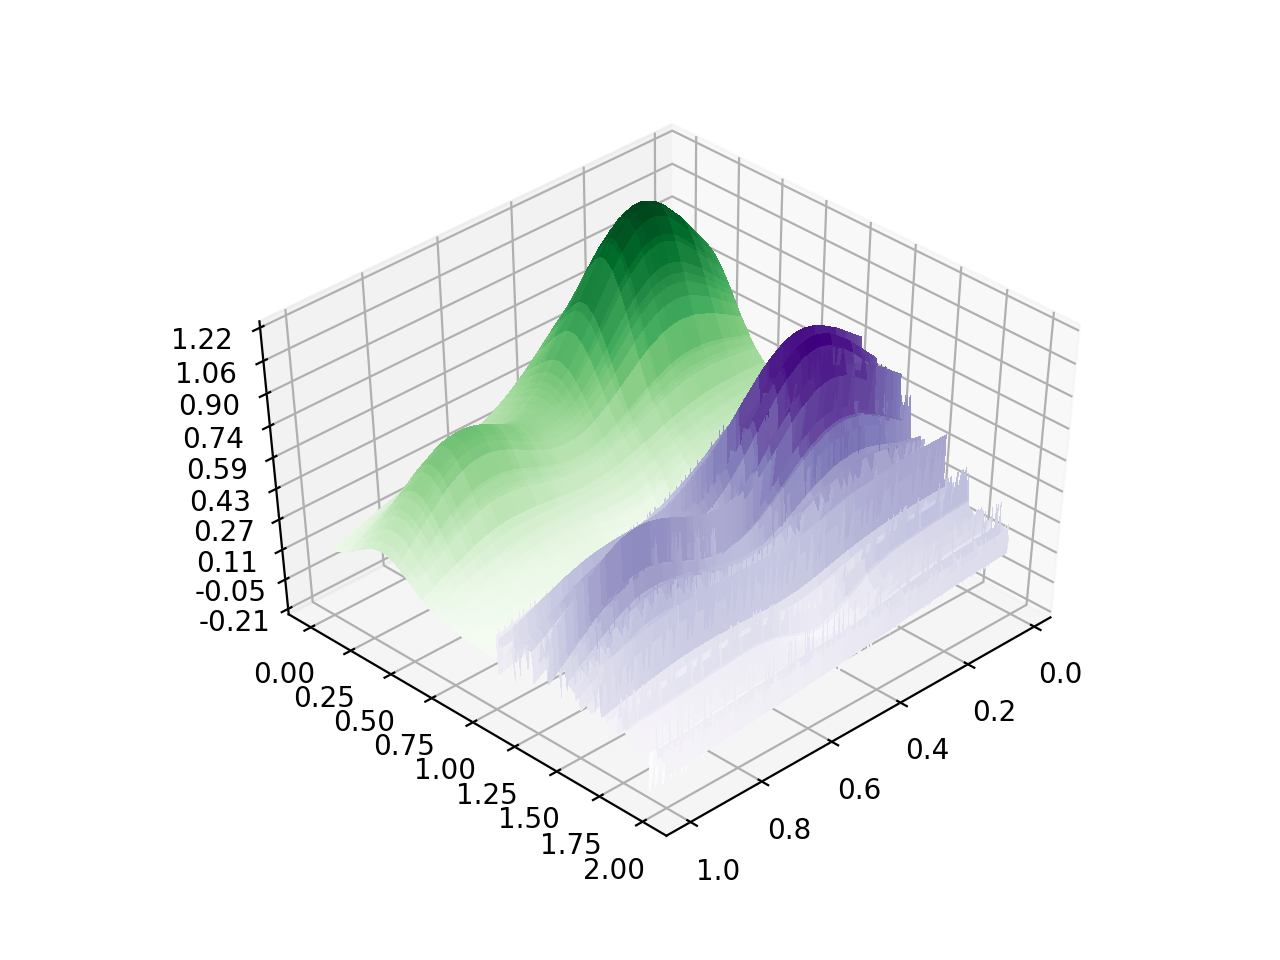
\includegraphics[width=\linewidth]{result/bilder/Franke_noise.png}
        	\caption{}
     \end{subfigure}
     ~
     \begin{subfigure}{0.45\textwidth}
       	\centering
       	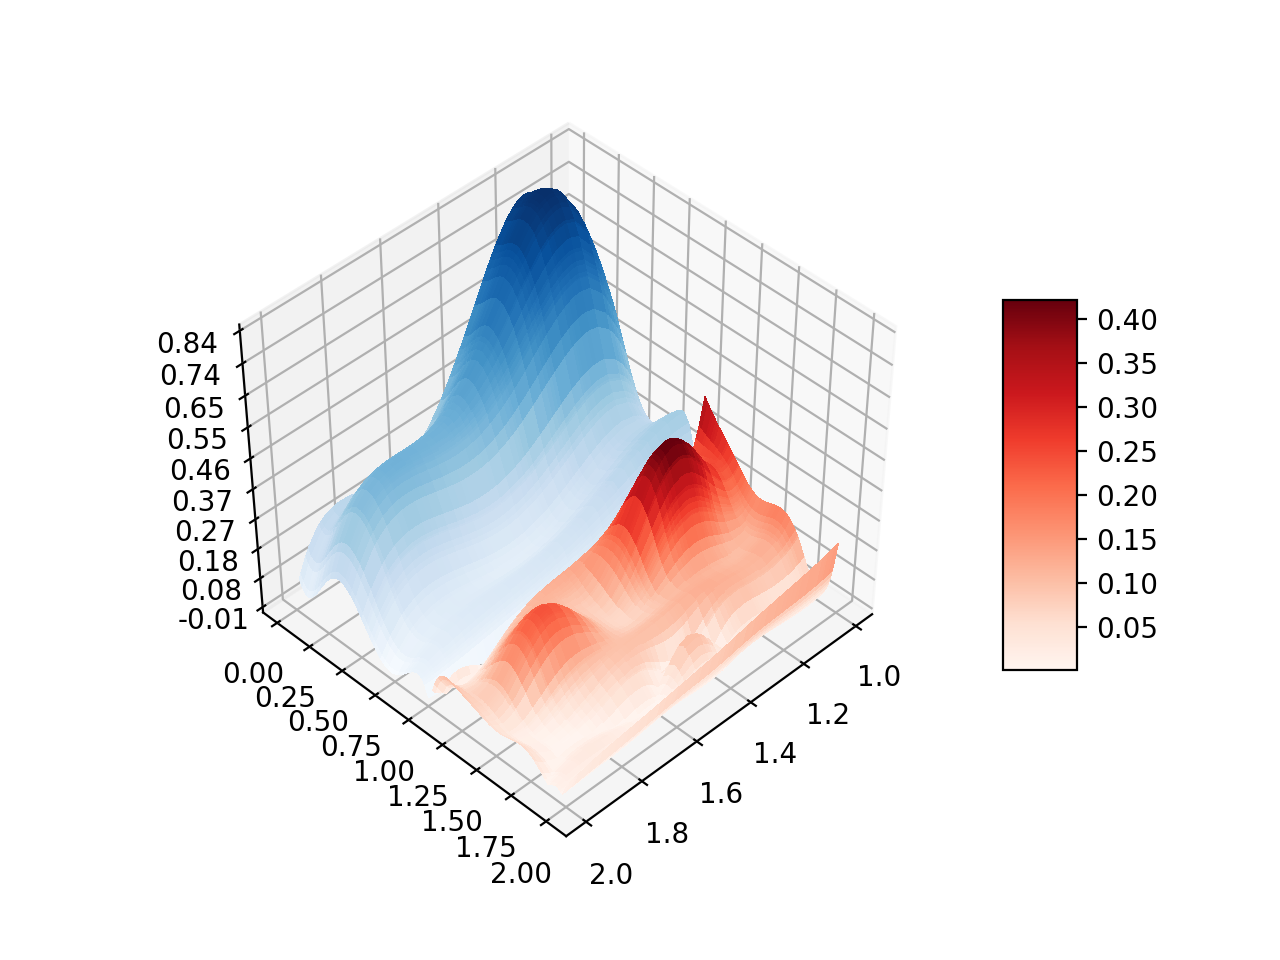
\includegraphics[width=\linewidth]{result/bilder/OLS_bar.png}
        	\caption{}
    	\end{subfigure}
 	\caption{a) \color{green}Franke function \color{black}, and the \color{purple}Frank function with noise plottet\color{black}. b) Our \color{blue}fifth order approximation of the Franke function\color{black}. On the right we have the \color{red}residuals\color{black}, i.e. the error compared to the real function, and its relative size indicated by the red colour gradient.}
	\label{fig:OLS_Frank}
\end{figure}


 \begin{center}
 \label{tab:OLS_Degree_R2_MSE}
 \captionof{table}{MSE and $R^2$ score for OLS by degree. These values are created by taking the average values over 100 different executions, with a noise level $= 0.1$ and a $\lambda = 0.00001$ }
 \begin{tabularx}{\textwidth}{c X c X c  }
     \hline
     \hline
         Degree && R2 && MSE \\
         \hline
2      && 0.71 && 0.01353 \\ 
3      && 0.81 && 0.00916 \\ 
4      && 0.86 && 0.00712 \\ 
5      && 0.88 && 0.00585 \\ \hline
 \end{tabularx}
 \end{center}
 
 \pagebreak
 \begin{center}
 \label{tab:OLS_lambda_R2_MSE}
 \captionof{table}{ MSE and $R^2$ score for OLS by $\lambda$, with a fifth order polynomial. These values are created by taking the average values over $100$ different executions, with a noise level $= 0.1$}
 \begin{tabularx}{\textwidth}{c X c X c  }
     \hline
     \hline
         $\lambda$ && R2 && MSE \\
         \hline
 0.0000001  && 0.87497  && 0.00587 \\
0.0000100  && 0.87517  && 0.00605 \\
0.0010000  && 0.87723  && 0.00592 \\
0.1000000  && 0.87242 && 0.00608 \\
1.0000000  && 0.87708 && 0.00613 \\
2.0000000  && 0.87833 && 0.00586 \\
5.0000000  && 0.87572 && 0.00601 \\
10.0000000 && 0.87528 && 0.00591\\ \hline
 \end{tabularx}
 \end{center}

  \begin{center}
 \label{tab:Confidenceintervall_OLS}
 \captionof{table}{$\beta$, Var and Confidence intervall for OLS by degree of $x$ and $y$. }
 \begin{tabularx}{\textwidth}{c X l X l X l }
     \hline
     \hline
     $x^iy^j$ && $\beta$ && VAR && Confidence intervall \\
     \hline
$x^0y^0$     && 0.259   && 0.001   &&  [0.227, 0.291]     \\ 
$x^0y^1$     && 4.117   && 0.108   &&  [3.788, 4.446]     \\ 
$x^0y^2$     && -18.065 && 2.943   &&  [-19.781, -16.349] \\ 
$x^0y^3$     && 29.764  && 15.934  &&  [25.772, 33.756]   \\ 
$x^0y^4$     && -22.199 && 17.571  &&  [-26.391, -18.007] \\ 
$x^0y^5$     && 6.361   && 2.637   &&  [4.737, 7.985]     \\ 
$x^1y^0$     && 5.277   && 0.074   &&  [5.005, 5.549]     \\ 
$x^1y^1$     && -9.751  && 1.234   &&  [-10.862, -8.64]   \\ 
$x^1y^2$     && 13.591  && 6.186   &&  [11.104, 16.078]   \\ 
$x^1y^3$     && -21.609 && 7.858   &&  [-24.412, -18.806] \\ 
$x^1y^4$     && 12.635  && 1.628   &&  [11.359, 13.911]   \\ 
$x^2y^0$     && -22.726 && 1.825   &&  [-24.077, -21.375] \\ 
$x^2y^1$     && 28.964  && 5.900   &&  [26.535, 31.393]   \\ 
$x^2y^2$     && -1.849  && 6.149   &&  [-4.329, 0.631]    \\ 
$x^2y^3$     && -5.401  && 1.364   &&  [-6.569, -4.233]   \\ 
$x^3y^0$     && 30.056  && 10.123  &&  [26.874, 33.238]   \\ 
$x^3y^1$     && -36.035 && 7.072   &&  [-38.694, -33.376] \\ 
$x^3y^2$     && 6.742   && 1.441   &&  [5.542, 7.942]     \\ 
$x^4y^0$     && -11.919 && 12.008  &&  [-15.384, -8.454]  \\ 
$x^4y^1$     && 12.813  && 1.444   &&  [11.611, 14.015]   \\ 
$x^5y^0$     && -0.909  && 1.951   &&  [-2.306, 0.488]    \\ 

     \hline
 \end{tabularx}
 \end{center}

 
\subsubsection{Ridge regression}
The results from the Ridge calculations are here presented in the same manner as for Ordinary least square. Again finding the MSE, $R^2$ score, according to polynomial degree, and testing for different $\lambda$. Finding the $\beta$ values, VAR, and the Confidence intervall. We see here that the $R^2$ score is unstable for higher values of $\lambda$.
 
 \pagebreak
 \begin{center}
 \label{tab:Ridge_Degree_R2_MSE}
 \captionof{table}{MSE and $R^2$ score for Ridge by degree. These values are created by taking the average values over 100 different executions, with a noise level $= 0.1$ and a $\lambda = 0.00001$.}
 \begin{tabularx}{\textwidth}{c X c X c  }
     \hline
     \hline
         Degree && R2 && MSE \\
         \hline
2      && 0.71 && 0.01353 \\ 
3      && 0.80 && 0.00968 \\ 
4      && 0.81 && 0.00928 \\ 
5      && 0.81 && 0.00902 \\ \hline
 \end{tabularx}
 \end{center}
 
 
\begin{center}
 \label{tab:OLS_lambda_R2_MSE}
 \captionof{table}{ MSE and $R^2$ score for Ridge $\lambda$. These values are created by taking the average values over $100$ different executions, with a noise level $= 0.1$.}
 \begin{tabularx}{\textwidth}{c X c X c  }
     \hline
     \hline
         $\lambda$ && R2 && MSE \\
         \hline
 0.0000001  && 0.81150  && 0.00894 \\
0.0000100  && 0.80979  && 0.00932 \\
0.0010000  && 0.74059  && 0.01237 \\
0.1000000  && -0.20901 && 0.05933 \\
1.0000000  && -1.85170 && 0.13474 \\
2.0000000  && -1.83823 && 0.14025 \\
5.0000000  && -1.79681 && 0.13813 \\
10.0000000 && -1.81950 && 0.13576\\ \hline
 \end{tabularx}
 \end{center}


  \begin{center}
 \label{tab:Confidenceintervall_Ridge}
 \captionof{table}{$\beta$, Var and Confidence intervall for Ridge by degree of $x$ and $y$. }
 \begin{tabularx}{\textwidth}{c X l X l X l }
     \hline
     \hline
     $x^iy^j$ && value && variance && Confidence intervall \\
     \hline
$x^0y^0$     && 0.384    && 0.001   && [0.352, 0.416]     \\
$x^0y^1$     && 1.770    && 0.077   && [1.493, 2.047]     \\
$x^0y^2$     && -0.294   && 1.953   && [-1.691, 1.103]    \\
$x^0y^3$     && -22.690  && 10.474  && [-25.926, -19.454] \\
$x^0y^4$     && 41.542   && 12.033  && [38.073, 45.011]   \\
$x^0y^5$     && -20.675  && 1.949   && [-22.071, -19.279] \\
$x^1y^0$     && 5.348    && 0.068   && [5.087, 5.609]     \\
$x^1y^1$     && -11.544  && 1.040   && [-12.564, -10.524] \\
$x^1y^2$     && 18.567   && 4.891   && [16.355, 20.779]   \\
$x^1y^3$     && -27.573  && 6.071   && [-30.037, -25.109] \\
$x^1y^4$     && 14.943   && 1.295   && [13.805, 16.081]   \\
$x^2y^0$     && -21.987  && 1.712   && [-23.295, -20.679] \\
$x^2y^1$     && 32.153   && 5.221   && [29.868, 34.438]   \\
$x^2y^2$     && -5.093   && 5.179   && [-7.369, -2.817]   \\
$x^2y^3$     && -3.142   && 1.161   && [-4.219, -2.065]   \\
$x^3y^0$     && 25.775   && 9.426   && [22.705, 28.845]   \\
$x^3y^1$     && -39.259  && 6.976   && [-41.9, -36.618]   \\
$x^3y^2$     && 6.673    && 1.214   && [5.571, 7.775]     \\
$x^4y^0$     && -4.833   && 11.244  && [-8.186, -1.48]    \\
$x^4y^1$     && 14.552   && 1.590   && [13.291, 15.813]   \\
$x^5y^0$     && -4.681   && 1.908   && [-6.062, -3.3]    \\ 
    \hline
 \end{tabularx}
 \end{center}      

 

\subsubsection{Lasso regression}
The results from the Lasso regression, again presenting the MSE, $R^2$, $\beta$, VAR, and Confidence interval.


 \begin{center}
 \label{tab:Lasso_Degree_R2_MSE}
 \captionof{table}{MSE and $R^2$ score for Lasso by degree. These values are created by taking the average values over 100 different executions, with a noise level $= 0.1$ and a $\lambda = 0.00001$}
 \begin{tabularx}{\textwidth}{c X c X c  }
     \hline
     \hline
         Degree && R2 && MSE \\
         \hline
2      && 0.71 && 0.01353 \\ 
3      && 0.81 && 0.00916 \\ 
4      && 0.86 && 0.00712 \\ 
5      && 0.88 && 0.00585 \\ \hline
 \end{tabularx}
 \end{center}
 
 
 \begin{center}
 \label{tab:Degree_R2_MSE}
 \captionof{table}{MSE and $R^2$ score for Lasso on Franke function by $\lambda$. These values are created by taking the average values over 100 different executions, with a noise level $= 0.1$}
 \begin{tabularx}{\textwidth}{c X c X c  }
     \hline
     \hline
$\lambda$    &&R2     &&MSE     \\
         \hline
0.0000001 &&0.87497&&0.00587 \\
0.0000100 &&0.87517&&0.00605 \\
0.0010000 &&0.87723&&0.00592 \\
0.1000000 &&0.87242&&0.00608 \\
1.0000000 &&0.87708&&0.00613 \\
2.0000000 &&0.87833&&0.00586 \\
5.0000000 &&0.87572&&0.00601 \\
10.0000000 && 0.87528&&0.00591
 \end{tabularx}
 \end{center}
 
 \begin{center}
\label{tab:lasso-var-conf}
\captionof{table}{$\beta$, Var and Confidence intervall for Ridge by degree of $x$ and $y$. We have here cut the values for higher degrees because these were equal to zero.}
\begin{tabularx}{\textwidth}{c X c X c X l}
    \hline
    \hline
        $x^iy^j$ && $\beta$ && VAR && Confidens interval\\
    \hline
        $x^0y^0$ && 0.342129   && 0.000080   && [0.333197,0.351061] \\
        $x^0y^1$ && -0.437389  && 0.000347   && [-0.456013,-0.418765] \\
        $x^0y^2$ && -0.016612  && 0.000261   && [-0.032765,-0.000458] \\
        $x^0y^5$ && 0.000024   && 0.000000   && [-0.000140,0.000188] \\
        $x^1y^0$ && 0.558845   && 0.000299   && [0.541543,0.576146] \\
        $x^1y^1$ && -0.389778  && 0.000394   && [-0.409623,-0.369933] \\
        $x^3y^0$ && -0.000178  && 0.000001   && [-0.000933,0.000576] \\
        $x^4y^0$ && -0.120878  && 0.000436   && [-0.141758,-0.099998] \\
    \hline
\end{tabularx}
\end{center}


 
\subsection{Ordinary least square, Ridge, and Lasso regression with resampling, now on real data}
In this section we present the OLS, Ridge and Lasso regression on the real data.
\begin{figure}[H]
		\centering
		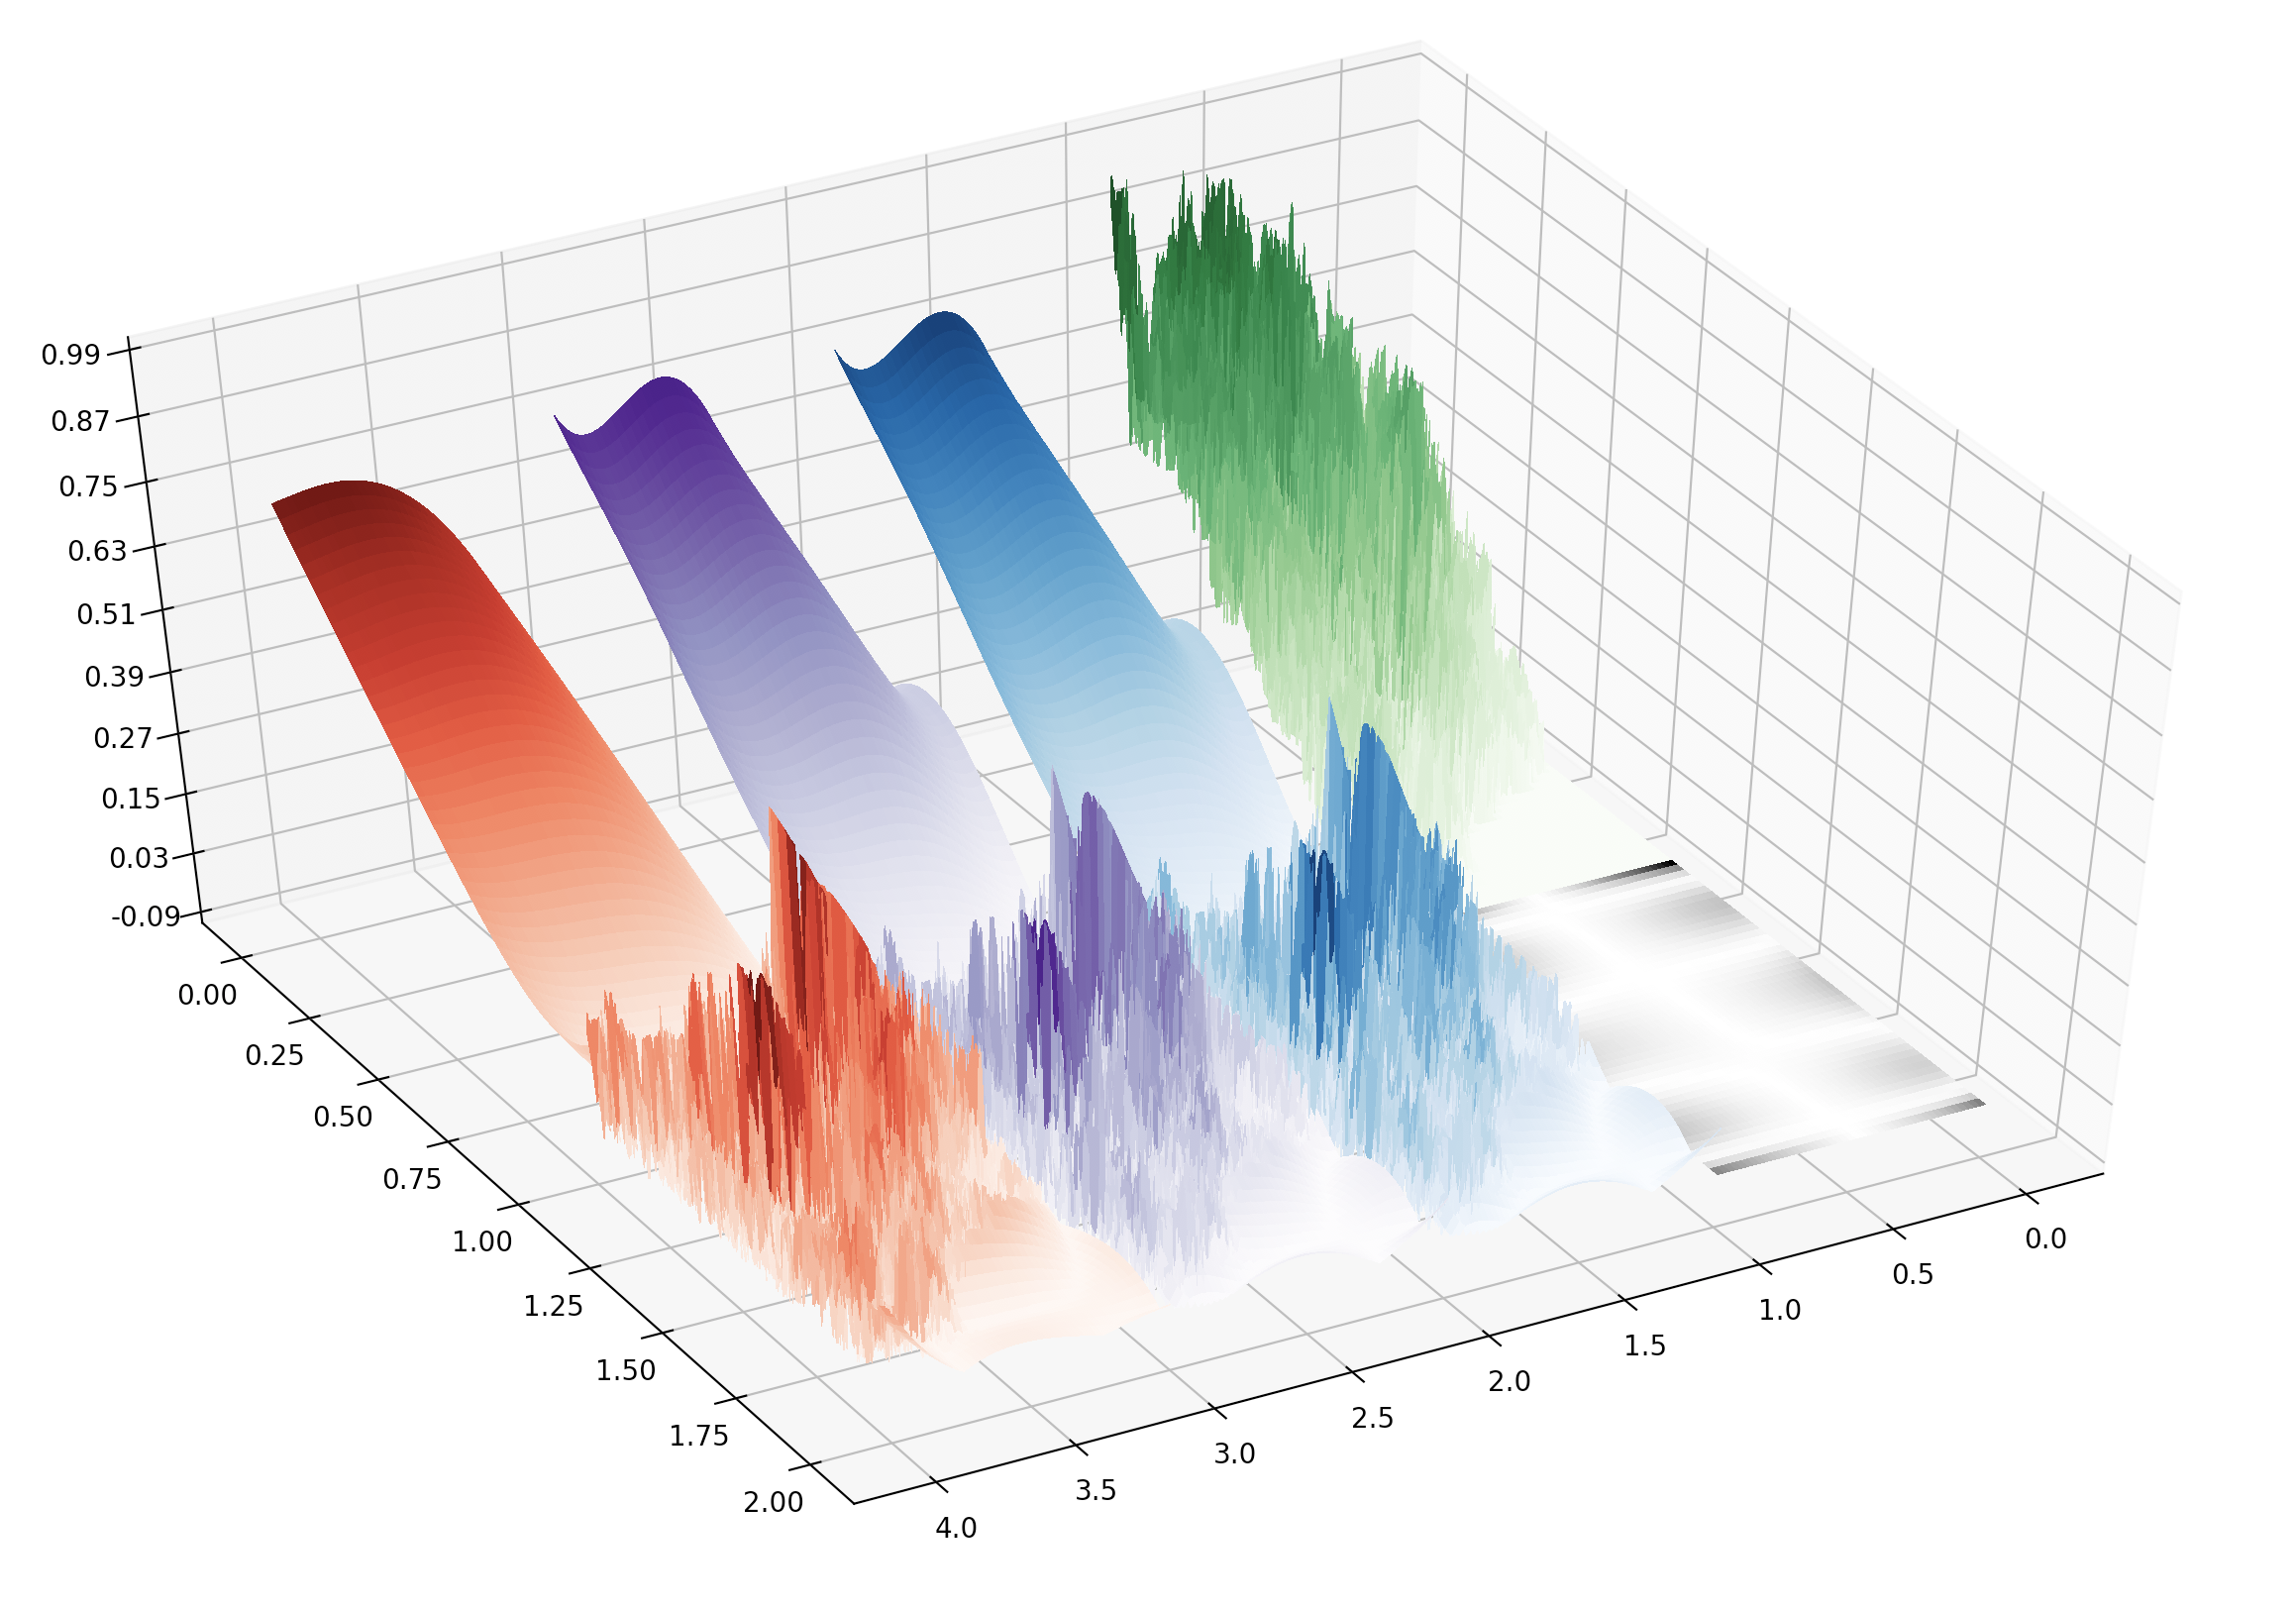
\includegraphics[width=1.1\linewidth]{result/bilder/all_real.png}
		\caption{From left to right: The \color{red}OLS \color{black} regression, \color{purple}{} Ridge \color{black} regression, \color{blue} Lasso \color{black} regression, and the \color{green}Real data \color{black} that we tried to approximate, with their residuals.}
		\label{fig:RealData}
\end{figure}


 \begin{center}
 \label{tab:Realdata_OLS_lambda_R2_MSE}
 \captionof{table}{OLS regression on Real data. }
 \begin{tabularx}{\textwidth}{c X c X c  }
     \hline
     \hline
$\lambda$    &&R2     &&MSE     \\
         \hline
0.0000001 && 0.823088 && 0.010720 \\
0.0000100 && 0.823088 && 0.010720 \\
0.0010000 && 0.823088 && 0.010720 \\
0.1000000 && 0.823088 && 0.010720 \\
 \end{tabularx}
 \end{center}
 
\pagebreak
 
 \begin{center}
 \label{tab:Realdata_Lasso_lambda_R2_MSE}
 \captionof{table}{Lasso on realdata. We saw that $R^2$ got out of hand with a $\lambda = 0.1$ and higher, and decided not to include those numbers. }
 \begin{tabularx}{\textwidth}{c X c X c  }
     \hline
     \hline
$\lambda$    &&R2     &&MSE     \\
         \hline
0.0000001 && 0.797486 && 0.012272 \\
0.0000100 && 0.797470 && 0.012273 \\
0.0010000 && 0.753280 && 0.014950 \\
0.1000000 && -0.165026 && 0.070596 \\
 \end{tabularx}
 \end{center}

 \begin{center}
 \label{tab:Realdata_Ridge_lambda_R2_MSE}
 \captionof{table}{Ridge on realdata. MSE and $R^2$ score for Ridge on the real data by $\lambda$. }
 \begin{tabularx}{\textwidth}{c X c X c  }
     \hline
     \hline
$\lambda$    &&R2     &&MSE     \\
         \hline
0.0000001 && 0.823088 && 0.010720 \\
0.0000100 && 0.823088 && 0.010720 \\
0.0010000 && 0.823027 && 0.010724 \\
0.1000000 && 0.818116 && 0.011022 \\
 \end{tabularx}
 \end{center}





%Presenter en kristisk vurdering og diskuter applikasjonsmulighetene(applicability) av disse regresjonsmetodene til typen data som blir presentert her. DISKUSJONSDEL





%\pagebreak
%\section{Discussion}
%\input{discussion/discussion}


\section{Conclusion}




It seems that the SIRS model is a great system dynamics model for representing real diseases, in general a great foundation to build on for predicting disease, in this case, and how they establish themselvs within the population. We have also seen that it is very versatile, with a few improvements tested out, and combined in this report. It was shown that a Monte Carlo simulation were a great way of approaching the differential equations in a more realistic manner, if given a large enough dataset. 


\printbibliography

\section{Appendix}\label{sec:appendix}
\subsection{Supervised Learning, some results:}
\begin{tabular}{|c|c|c|c|c|c|c|} \hline
func	&	node	&	epoch	&	step	&		MSE		&	R2	\\ 
\hline
swis	&	100 	&	100 	& 	01 		&	4301.860	&	-1.504686		\\ 
\hline
swis	&	100 	&	100 	& 	001		&	4383.970	&	-0.062676		\\ 
\hline
swis	&	100 	&	100  	& 	0001	&	18649.730	&	-1612.388089		\\ 
\hline
swis	&	100 	&	1000 	& 	01		&	5405.858	&	-0.947049		\\ 
\hline
swis	&	100 	&	1000	& 	001		&	4996.257	&	-1.148733		\\ 
\hline
swis	&	100 	&	1000	& 	0001	&	4068.276	&	-0.079732		\\ 
\hline
swis	&	100 	&	10000	& 	01		&	 5405.352	&	 -0.946243		\\ 
\hline
swis	&	100 	&	10000	& 	001		&	 5405.650	&	 -0.946284		\\ 
\hline
swis	&	100 	&	10000	& 	0001 	&	5395.676 	& -0.955657		\\ 
\hline
swis	&	1000	&	 100	& 	01		&	 5344.535	&	 -0.9690825\\ 
\hline
swis	&	1000	&	 100	& 	001		&	 4301.586	&	 -1.5146678\\ 
\hline
swis	&	1000	&	 100	& 	0001	&	 7687.034	&	 -7.0514296\\ 
\hline
swis	&	1000	&	 1000	& 	01		&	 5406.056	&	 -0.9465423\\ 
\hline
swis	&	1000	&	 1000 	& 	001		&	 5405.020	&	 -0.9540634\\ 
\hline
swis	&	1000	&	 1000 	&	 0001	&	 4381.460	&	 -1.5773855\\ 
\hline
swis	&	1000	&	 10000 	&  	01		&	 5408.282	&	 -0.9504758\\ 
\hline
swis	&	1000	&	 10000 	&	 001	&	 5405.543	&	 -0.9462314\\ 
\hline
swis	&	1000	&	 10000 	&	 0001	&	 5407.491	&	 -0.9473403\\ 
\hline
tan 	& 100 		&   100   	& 	01		&	 4722.055 	&	-1.4382791	\\ 
\hline
tan 	& 100  		&	100   	& 	001		&	 4541.822 	&	-63.0650826	\\ 
\hline
tan 	& 100  		&	100   	& 	0001	&	 18327.134	&	 -2164.3759400 	\\ 
\hline
tan 	& 100  		&	1000  	& 	01		&	 5389.155 	&	-0.9489306     \\
\hline
tan 	& 100  		&	1000  	& 	001		&	 4560.229 	&	-1.4495536   	\\ 
\hline
tan 	& 100  		&	1000  	&	 0001	&	 4609.627 	&	-47.9667788	\\ 
\hline
tan 	& 100  		&	10000 	& 	01 		&	5406.032	&	 -0.9464465	\\ 
\hline
tan 	& 100  		&	10000 	& 	001 	&	5405.054	&	 -0.9468466	\\ 
\hline
tan 	& 100  		&	10000 	& 	0001 	&	5136.405	&	 -1.0999677	\\ 
\hline
tan 	& 1000 		&	 100  	& 	01 		&	5301.474	&	 -1.0137502	\\ 
\hline
tan 	& 1000 		&	 100  	& 	001 	&	4726.264	&	 -1.5468762	\\ 
\hline
tan 	& 1000 		&	 100  	& 	0001 	&	6837.188 	&	-10.2774431	\\ 
\hline
tan 	& 1000 		&	 1000 	 & 	01		&	 5408.170	&	 -0.9473984	\\ 
\hline
tan 	& 1000 		&	 1000 	 & 	001 	&	5401.553 	&	-0.9657959\\ 
\hline
tan 	& 1000 		&	 1000 	 & 	0001	&	 4568.399	&	 -1.4008756\\ 
\hline
tan 	& 1000 		&	 10000	 & 	01		&	 5530.394	&	 -0.9048310\\ 
\hline
tan 	& 1000 		&	 10000	 & 	001		&	 5408.057	&	 -0.9453489\\ 
\hline
tan 	& 1000 		&	 10000	 & 	0001	&	 5408.827	&	 -0.9476682\\ 
\hline
arctan& 100 &100	& 01& 4695.224& -1.3245204	\\ 
\hline
arctan& 100 &100	& 001 &3061.016 & -6.1246861	\\ 
\hline
arctan& 100 &100	& 0001 &18306.907& -1982.2542040	\\ 
\hline
arctan& 100 &1000 	&01 &5353.242& -0.9334961	\\ 
\hline
arctan& 100 &1000	& 001 &4352.663& -1.4293472	\\ 
\hline
arctan& 100 &1000	& 0001 &3198.084& -5.7849874	\\ 
\hline
arctan& 100 &10000	& 01 &5409.115& -0.9443223		\\ 
\hline
arctan& 100 &10000	& 001 &5399.718& -0.9443793	\\ 
\hline
arctan& 100 &10000 	&	0001 &5029.071 &-1.0632415	\\ 
\hline
arctan& 1000& 100 	&01& 5102.813& -1.0711406	\\ 
\hline
arctan& 1000& 100 	&001 &4579.046& -1.4685736	\\ 
\hline
\end{tabular}

See github.come/sondrt/





% \begin{figure}[H]
%     \centering
%     \begin{subfigure}{0.5\textwidth}
%         \centering
%         \includegraphics[width=\linewidth]{result/bilder/...}
%         \caption{}
%     \end{subfigure}%
%     ~
%     \begin{subfigure}{0.5\textwidth}
%         \centering
%         \includegraphics[width=\linewidth]{result/bilder/...}
%         \caption{}
%     \end{subfigure}
%     \caption{a)... b)...}
%     \label{fig:test}
% \end{figure}




% \begin{center}
% \label{tab:test}
% \captionof{table}{}
% \begin{tabularx}{\textwidth}{c X c X c X c }
%     \hline
%     \hline
%         $L_i$ && $T_C(L_i)$ && $T_C(\infty)$ with $\overline{a}$ \\
%     \hline
%         60      &&  2.30  && 2.2999\\
%         100     &&  2.29  && 2.2899\\
%         140     &&  2.28  && 2.2799\\
%         200     &&  2.27  && 2.2699\\
%     \hline
% \end{tabularx}
% \end{center}









%\begin{align*}
%&n \qquad &2^n - (-1)^n\\
%&n+1 \qquad &2^{n+1} - (-1)^{n+1} \\
%& &= 2(2^{n}) - (-1)^{n+1}\\
%& &= 2(2^{n} + (-1)^n  + (-1)^{n+1}) - (-1)^{n+1}\\
%& &= 2(2^{n} + (-1)^n  - (-1)^{n}) - (-1)^{n+1}\\
%& &= 2(2^{n}- (-1)^{n}) + 2(-1)^n  + (-1)^{n}\\
%& &= 2(2^{n}- (-1)^{n}) + 3(-1)^n \\
%\end{align*}


%\begin{figure}[H]
%		\centering
%		\includegraphics[width=0.7\linewidth]{ab.png}
%		\caption{Atomene er gule kuler, de elementære vektorene er blå og a vektorene er grønne.}
%		\label{fig:ab}
%\end{figure}

%\begin{tabular}{|c|c|c|c|c|c|c|}
%	\hline
%	n & General & Specific & LU & fastest & slowest & $\frac{slowest}{fastest}$\\
%	\hline
%	10 & 6.5e-05 & 5e-06 & 4e-05 & Specific & General & 13.0\\
%	\hline
%	100 & 7.5e-05 & 8e-06 & 0.0023 & Specific & LU & 287.5\\
%	\hline
%	1000 & 0.00014 & 4e-05 & 0.26 & Specific & LU & 6500\\
%	\hline
%	10000 & 0.0007 & 0.0005 & 142.5 & Specific & LU & 285000 \\
%	\hline
%\end{tabular}


\end{document}
